\chapter{Aspektorientierte Programmierung}
\label{chap:aop}

\section{Geschichte}
\label{sec:aop_geschichte}

Das Konzept der Aspektorientierten Programmierung wurde im Xerox PARC (Palo Alto Research Center Incorporated) entwickelt und gewann ab 1995 an Wichtigkeit. Wie bei allen neuen Spezifikationen war der Umfang und die Bestandteile der Aspektorientierten Programmierung zuerst nicht klar abgegrenzt. Gregor Kiczales und sein Team waren massgeblich an der Entwicklung von AOP beteiligt.\\
Nach Entwicklung des theoretischen Grundlage folgte im Jahre 1998 eine erste Version von AspectJ, eine Implementation von AOP in Java. Die Version 1.0 von AspectJ wurde jedoch erst im Jahre 2002 nach weiterer Forschung veröffentlicht.\cite{lopes:historyaop} \\
Die Aspektorientierte Programmierung wurde durch die Publikation von AspectJ bekannt und es wurden seither Erweiterungen für die meisten populären Programmiersprachen entwickelt. 

Die Entwicklung und der Betrieb von AspectJ wurde von XeroX Parc an Eclipse weitergereicht. Dort läuft AspectJ bis heute als Open-Source Projekt weiter. Mit der Version 1.8.7 wurde am 9. September 2015 die aktuellste Version veröffentlicht.

\section{Motivation}
\label{sec:aop_motivation}

Einer der Hauptgründe warum AOP entwickelt wurde ist die erweiterte Modularität die damit erreicht werden kann. Beim Design eines Systems werden in der Regel verschiedene Kategorien von Funktionalitäten aufgestellt und so die Software in verschiedene sogenannte Anliegen aufgeteilt. Dabei unterscheidet man zwischen den folgenden zwei Gruppen:

\begin{itemize}
	\item Kernanliegen (core concerns)\\
	Hierbei handelt sich um die Kernfunktionalität der Applikation, die sogenannte Business Logic. Diese Gruppe beinhaltet zum Beispiel den Datenbankzugriff, die Interagierung mit dem Benutzer etc.
	\item System Übergreifende Anliegen (cross-cutting concerns) \\
	Andere Funktionalitäten wie das Logging, die Sicherheit, Concurrency sowie Transaktionen betreffen das gesamte System.
\end{itemize}

Diese Gruppen dienen als Grundlage zur Veranschaulichung, warum gerade bei der Modularisierung die OOP Schwachstellen aufweist.\newpage

\subsection{Objektoriente Programmierung}
\label{sec:aop_oop}

Mit der Objektorientierten Programmierung wurden viele Probleme und Unschönheiten von Prozeduralen Sprachen gelöst. Die OOP besitzt riesige Vorteile, welche die Softwareentwicklung vereinfachen. Einige der Kernbestandteile von OOP sind:

\begin{itemize}
	\item Encapsulation: Daten und Methoden zur Veränderung derjenigen werden in Objekten gekapselt
	\item Inheritance: Das Verhalten oder die Daten können von einer Klasse geerbt werden.
	\item Polymorphism: ....
\end{itemize}

Die OOP erlaubt es Code modular zu strukturieren und Daten zu kapseln. Mit steigender Komplexität jedoch wird es schwierig den Code klar zu trennen und Abhängigkeiten so klein wie möglich zu halten.\\

Die Kernanliegen der Applikation werden in Klassen der Business Logic abgebildet. Diese Klassen werden jedoch sehr schnell durch den Code der System übergreifenden Anliegen "verschmutzt", so dass eine Klasse nicht nur für ein Anliegen verantwortlich ist. Dadurch wird das Single Responsibility Principle verletzt. Die folgende Graphik zeigt eine solche Beispielklasse, welche das beschriebene Phänomen veranschaulichen soll. Nur ein kleiner Teil der Methode (rot markiert) beschäftigt sich mit der Ausführung des Kernanliegens dieser Klasse, der Rest mit den System übergreifenden Anliegen.

\begin{figure}[H]
	\centering
		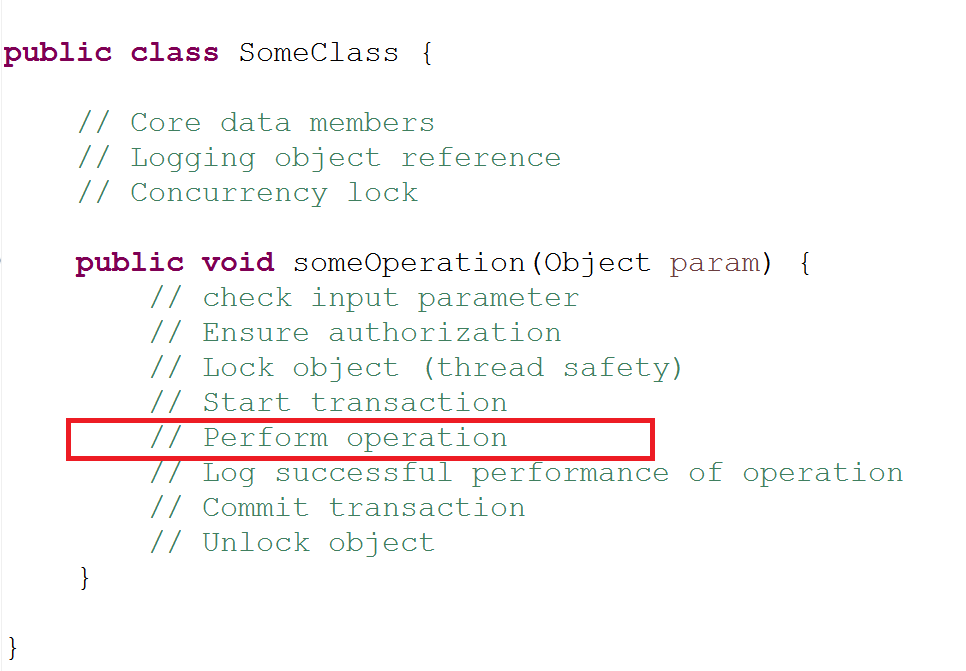
\includegraphics[scale=1.0]{bilder/motivationprogram.png}
	\caption{Beispielsklasse - Motivation für AOP}
	\label{fig:classmotivationaop}
\end{figure}



\paragraph{Code Tangling}

Von Code Tangling (to tangle - sich verwickeln) spricht man wenn ein Modul verschiedene Anliegen bearbeitet. Als Beispiel kann man die Abbildung \ref{fig:classmotivationaop} nehmen. Während der Designphase werden die Anliegen seperat entworfen und in der Implementation werden alle Funktionen verwickelt.

\paragraph{Code Scattering}

Bei Code Scattering (to scatter - streuen) ist die Perspektive eine andere. Die Funktionen eines Moduls werden in verschiedene anderen Modulen verwendetet und so im ganzen System gestreut. Folgende Abbildung soll dies anhand eines Sicherheitsmoduls veranschaulichen.

\begin{figure}[H]
	\centering
		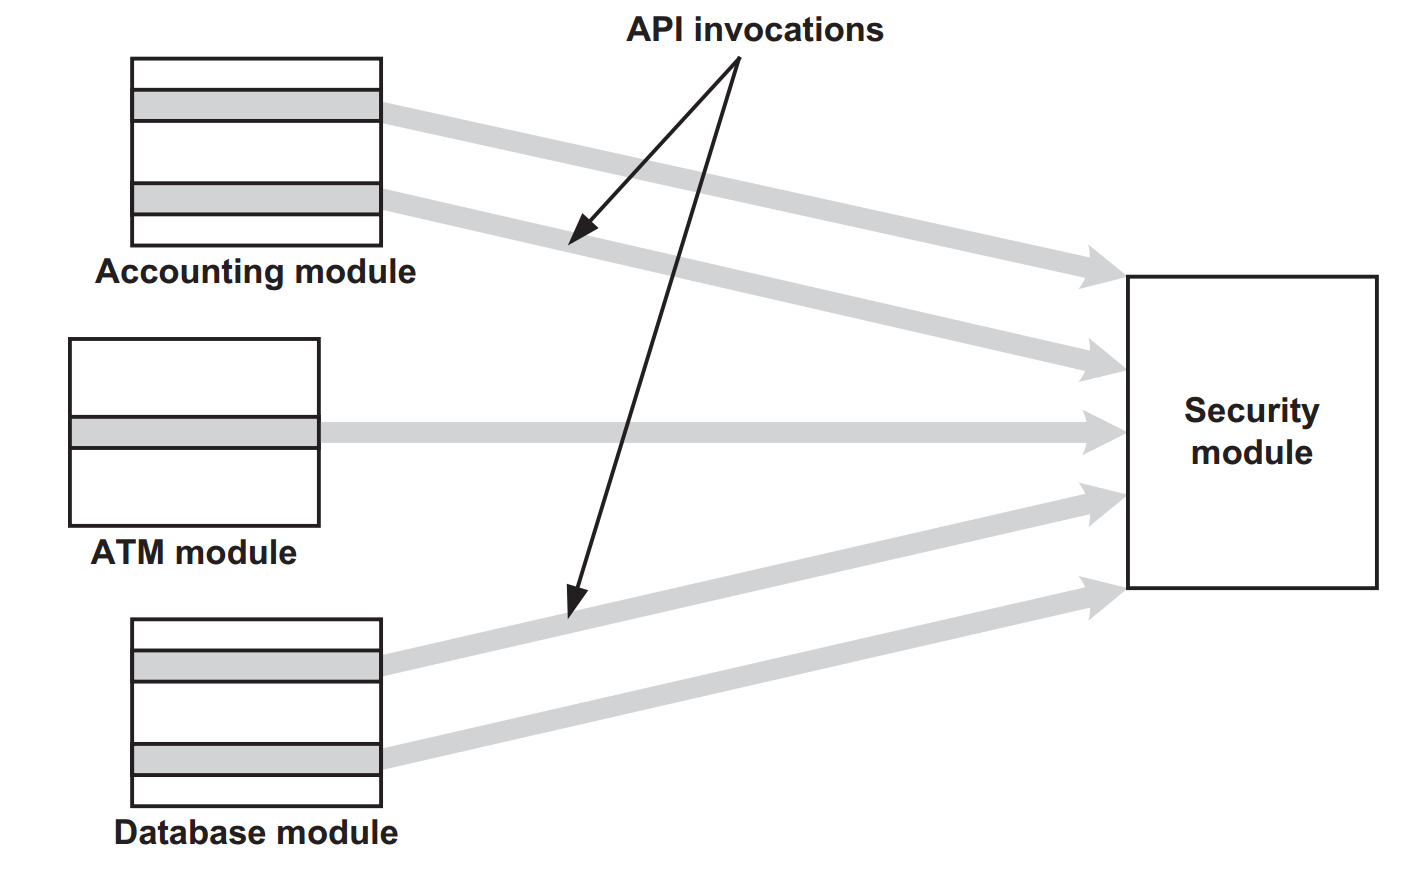
\includegraphics[scale=0.5]{bilder/motivationsCodeScattering.png}
	\caption{Code Scattering (Source \cite[p~54]{laddad:aspectj})}
	\label{fig:motivationcs}
\end{figure}

Bei Verwendung von OOP ist das Code Tangling und Code Scattering unumgänglich. Selbst bei einem perfekt designten System werden diese Phänomene vorhanden sein. Dies beeinflusst Software Design und Entwicklung auf vielerlei Arten: Schlechte Nachvollziehbarkeit, weniger Produktivität, weniger Wiederverwendbarkeit von Code, viele repetitive Arbeiten, schlechtere Qualität und Wartbarkeit von Applikationen. Aus diesen Gründen macht es Sinn nach Alternativen zu suchen, ohne jedoch auf die Vorzüge von OOP zu verzichten.

\subsection{Modularisierung mit AOP}
\label{sec:aop_modaop}
Bleiben wir beim Beispiel eines Security Moduls; Das Modul wird mit Klassen implementiert und mittels Interfaces gegen aussen sichtbar gemacht. In der OOP werden nun alle Codeteile welche Securityfunktionen verwenden möchten einen Aufruf dieses Moduls beinhalten. Bei einer Änderung in der API müssen unter Umständen tausende Aufrufe ebenfalls geändert werden. Mit AOP jedoch beinhalten die Client Module keine Aufrufe mehr. Aufrufe des Sicherheitsmoduls werden bei genau definierten Punkten im Code automatisch ausgelöst. Als Beispiel kann definiert werden, dass bei allen öffentlichen Methoden einer Klasse vor Ausführung des Bodys die Berechtigung des Benutzers geprüft wird. Bei dieser Deklaration der Einstiegspunkte im Code und des in diesen Fällen auszuführenden Codes spricht man von einem Aspect. Um diese automatische Ausführung möglich zu machen muss der Code mit dem des Aspects verwebt werden. Man spricht hierbei von Weaving.
\begin{figure}[H]
	\centering
		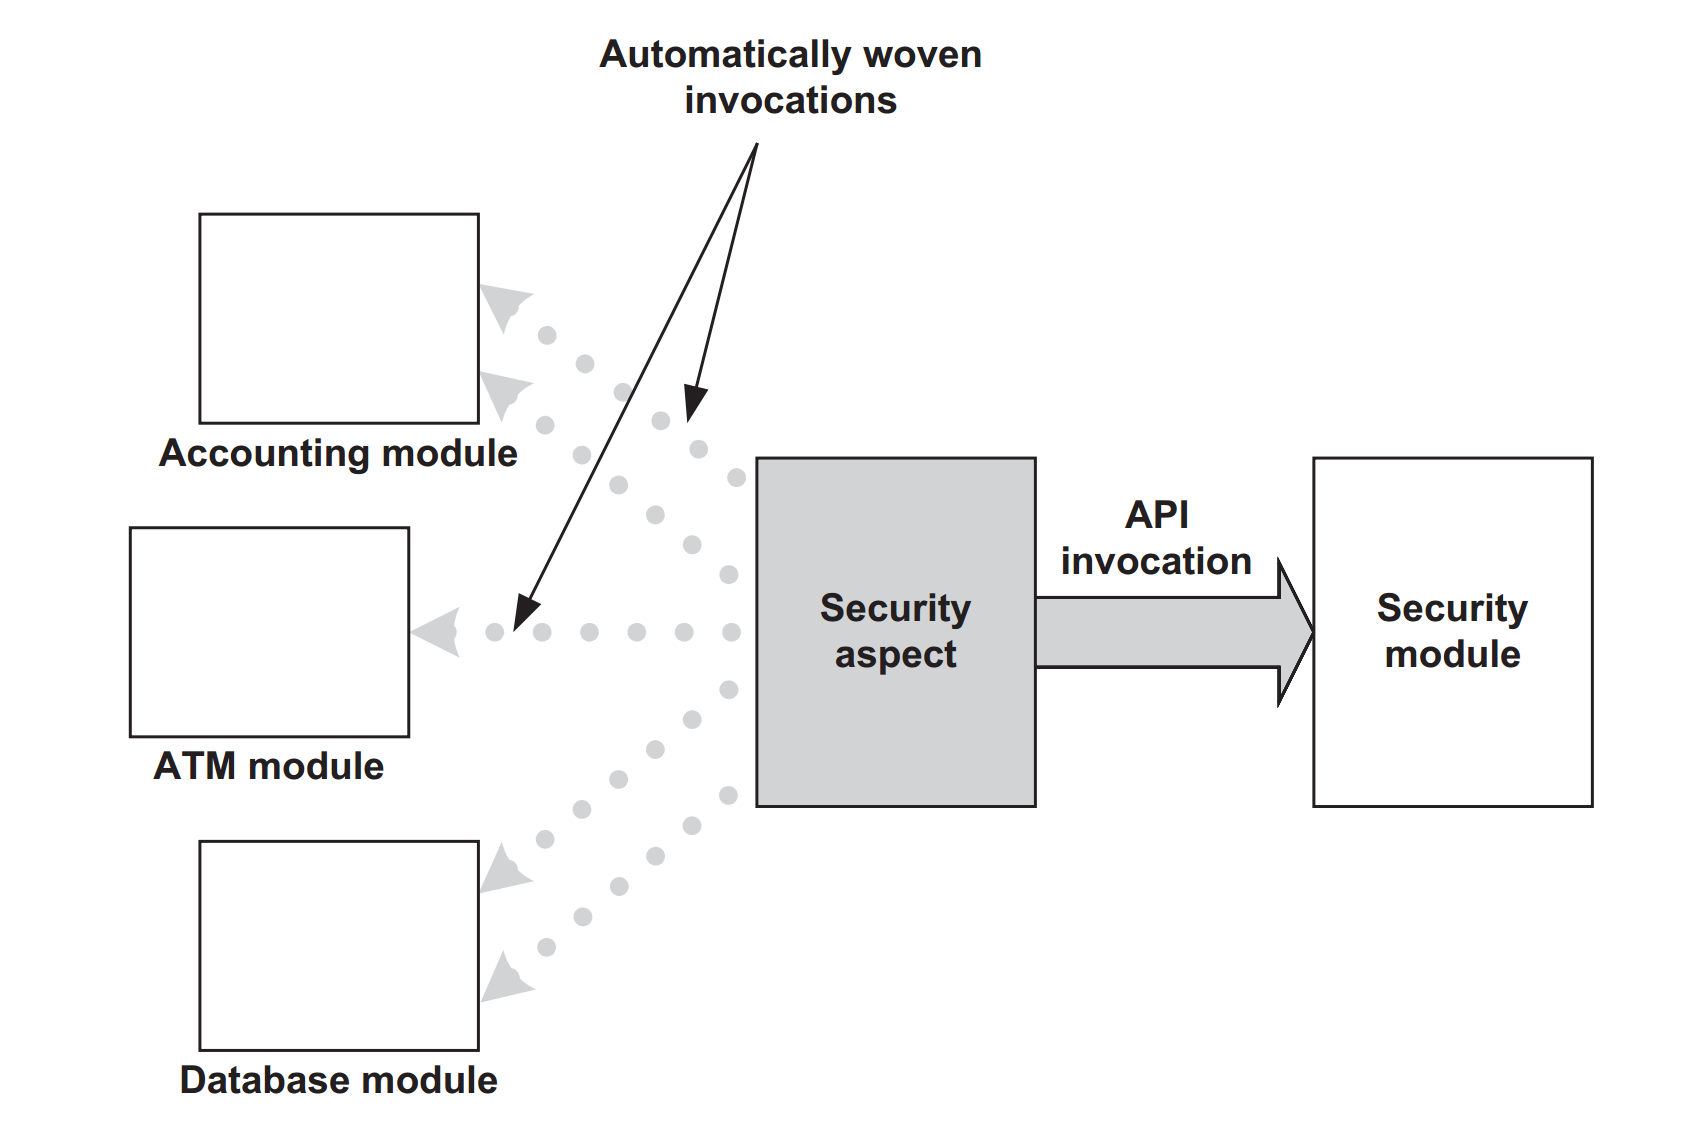
\includegraphics[scale=0.5]{bilder/motivationAop.png}
	\caption{Systemdesign mit AOP (Source\cite[p~55]{laddad:aspectj})}
	\label{fig:motivationaop}
\end{figure}

\section{Aspektorientierte Sprache}
\label{sec:aop_lang}
Die Aspektorientierte Programmierung ist eine Methode und muss um verwendet werden zu können spezifiziert und danach implementiert werden.
\subsection{Spezifizierung}
\subparagraph{Programmiersprache}
Als Grundlage für die Entwicklung eines Aspektorientierten Programms dient eine Programmiersprache. Es werden in der Regel bestehende Programmiersprachen wie C, C++, CSharp und Java verwendet. Mit dieser Sprache werden die einzelnen Module unabhängig entwickelt ohne auf einander zuzugreifen.
\subparagraph{Weaving Rules Spezifizierung}
Die Sprache muss eine Möglichkeit bieten um diese entwickelten Module miteinander verknüpfen zu können. Dazu müssen sogenannte Weaving Rules deklariert werden. Die Weaving Rules bestimmen wie der Code verknüpft wird. Hierfür können Standardelemente einer Sprache verwendet werden (Annotations) oder auch die bestehende Sprache um neue Elemente erweitert werden (Keywords).
\subsection{Implementation}
Eine Implementation einer AOP Sprache kann in zwei Schritte gegliedert werden. Zuerst werden die verschiedenen Anliegen mittels Weaving rules verknüpft und daraus anschliessend ausführbarer Code konvertiert.
Ein sogenannter Weaver führt diese Aufgaben aus. Es gibt drei verschiedene Typen von Weavern:

\begin{itemize}
\item Source-to-Source \\ Der Sourcecode der Core und Crosscutting concerns wird zuerst verwoben und dieser neu entstandene Source Code von einem regulären Compiler kompiliert. 
\item Byte Code \\ Der Sourcecode der Core und Crosscutting concerns wird zuerst kompiliert und der daraus entstandene Byte Code wird vom Weaver verknüpft.
\item Load time \\ Vergleichbar mit dem Byte Code weaving, ausser dass der Verknüpfungsvorgang erst beim Aufrufen des Programms statt findet.
\end{itemize}

\section{Konzepte}

\begin{itemize}
\item Identifizierbare Punkte in der Ausführung des Systems
\item Selektion der gewünschten Punkte
\item Veränderung des regulären Programmablaufs
\item Veränderung der statischen Struktur des Systems
\item Ort zur Deklaration
\end{itemize}

\section{Programmiersprachen}

\paragraph{Java}

\paragraph{.NET Framework}

\paragraph{C++}
